\chapter{\rustsec{}: An SeKVM Rust Rewrite}
\label{sec:rewrite}

%We want to rewrite SeKVM in Rust.
%We first forward port SeKVM from 4.18 to 5.15, this is to use newer features
%e.g. LTO.
%Then we employ the two pass method.

Our goal is to enhance the security of the trusted \secore{} in SeKVM by
rewriting it in Rust. We first forward ported SeKVM from its original
Linux 4.18 version to the newest long term support version Linux 5.15 at the
time of development.
By forward porting we benefit from Linux's advancements including performance
optimizations such as Link-Time-Optimization (LTO) and energy aware scheduling.
And new kernel security features including \code{clang} shadow call stacks,
branch target identification, control flow integrity (CFI), ARM Memory Tagging
Extension (MTE), ARM pointer authentication, and randomized stack offset per
syscall.

%to take advantage of various new kernel features, for
%example  for better performance, ARM Pointer Authentication (5.0), Energy Aware Scheduling (5.0)
%clang shadow call stack, branch target identification (5.8), MTE (5.10), clang CFI (5.13), randomized stack offset per syscall (5.13)

Once the forward port of SeKVM to Linux 5.15 is ready, we can finally rewrite
the implementation in Rust.
This chapter describes the challenges that arose when trying to rewrite
\secore{} in Rust, and the techniques we employed to solve them.

\section{Integration with Linux}

%challenge: Linux 5.15 does not include Rust support
%
%solution: our way of source code organization, build system integration,
%how we link Rust and C, data layout issues, etc.

Linux 5.15, which is the latest long term support kernel version at the time of
\rustsec{} development, does not support Rust as a development language.
Therefore, we had to integrate Rust code with the rest of the Linux kernel.
We implement \rustcore{} in a single crate on the \code{no\_std} environment
and compile it into a single static library. The static library is then linked
with the rest of the kernel to create the final kernel image.
KVM separates EL2 code from EL1 by grouping EL2 code in a section
\code{.hyp.text}, then mapping that section in EL2's address space at
initialization.
In \rustcore{}, attribute \code{\#[link\_section = ".hyp.text"]} is prepended
to all code that should be run in EL2, so that they get placed in the
\code{.hyp.text} section as well.
Our implementation is compatible with the Linux kernel codebase. For example, we
ensure the page size definition is identical in \rustcore{} and KVM.
Also, we share types like \code{kvm\_vcpu} between Linux and \rustcore{}.
These type definitions are generated automatically
with the tool \code{bindgen}~\cite{bindgen}.
For constants that are used by both Linux and \rustcore{},
we copy them from C to Rust manually.
Due to the limited support of macro in \code{bindgen}
and the heavy usage of Linux,
we do not use it to generate constants.
Regarding alignment, field layout order, and padding of custom types,
Rust provides an attribute \code{\#[repr\-(C)]}
that ensures the data layout of the marked type has the same layout as in C.

\section{Bringing up \rustsec{} on Real Hardware}

We chose the Raspberry Pi model 4B (Rpi-4B) to verify our implementation on
real hardware.
%This section describes the problem that occured when trying to run SeKVM on
%Rpi-4B, and how we solved the issue.
SeKVM's trusted core \secore{} originally reserved its private memory by
defining global symbols whose addresses reside right after the kernel image,
in the Linux kernel linker script.
\secore{} then references those symbols to access and utilize the reserved
memory.
However, there exists an unusable hole in Rpi-4B's physical memory address
space, and the bootloader of Rpi-4B places the kernel image before the hole,
resulting in an overlap of \secore{}'s private memory and the unusable hole
(\autoref{fig:overlap}). This makes SeKVM unable to initialize on Rpi-4B.

\begin{figure}[hbtp]
    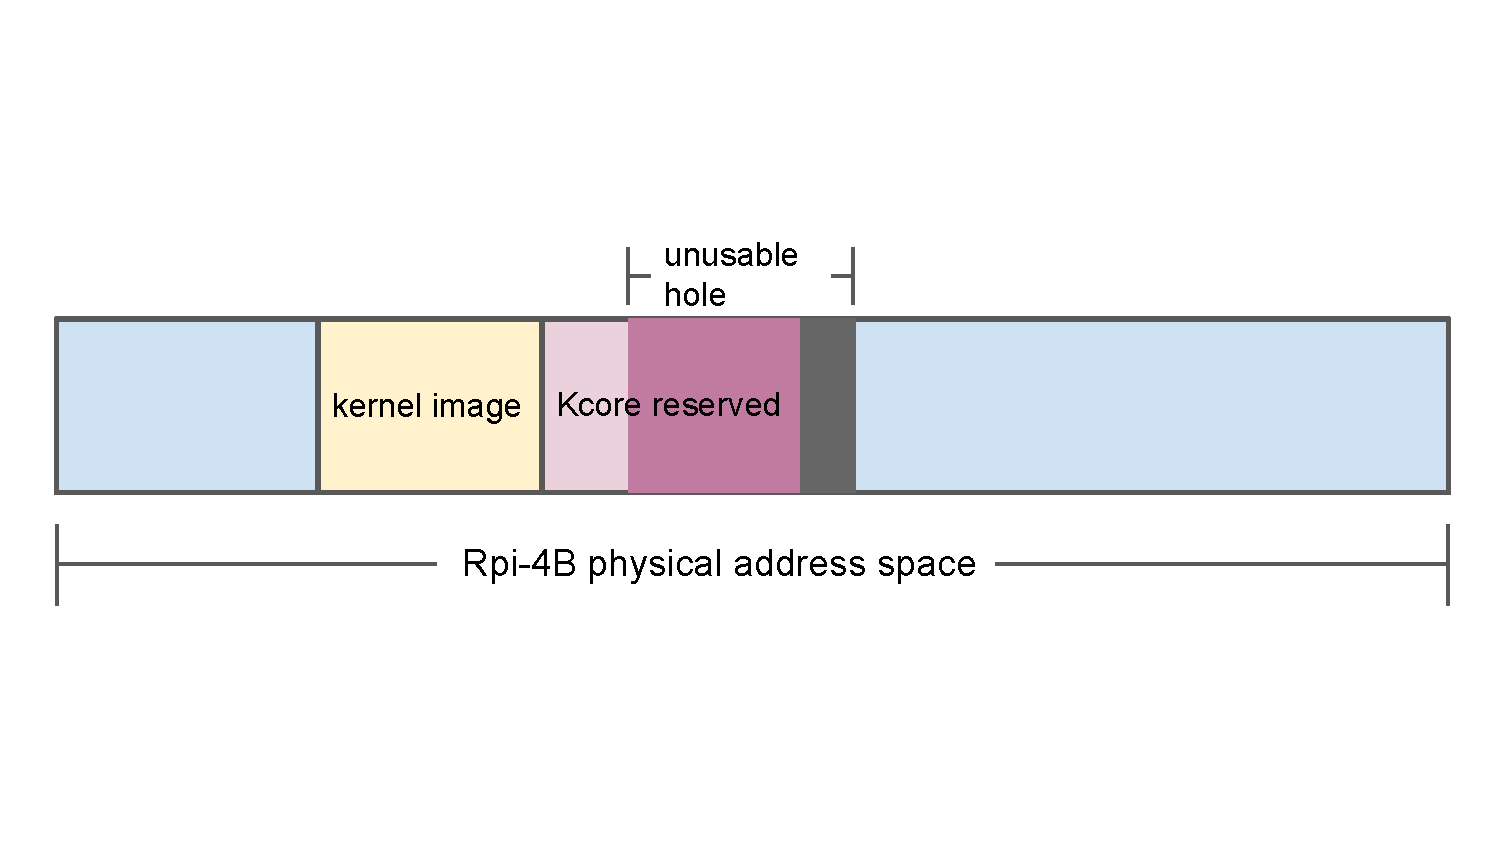
\includegraphics[scale=0.60]{figures/overlap.pdf}
    \caption{Kcore overlaps the unusable hole on Rpi-4B}
    \label{fig:overlap}
\end{figure}

To solve this issue, instead of allocating memory in the linker script,
we first locate a range of memory which does not overlap with the unusable hole
of Rpi-4B and the kernel image, then call \code{memblock\_reserve} to
mark the range of memory as reserved so that the kernel does not accidentally
access this memory range (\autoref{fig:rcorereserved}).
The global symbols have also been changed to C macros that expand into
addresses in the reserved range for \rustsec{}'s \rustcore{} usage.

\begin{figure}[H]
    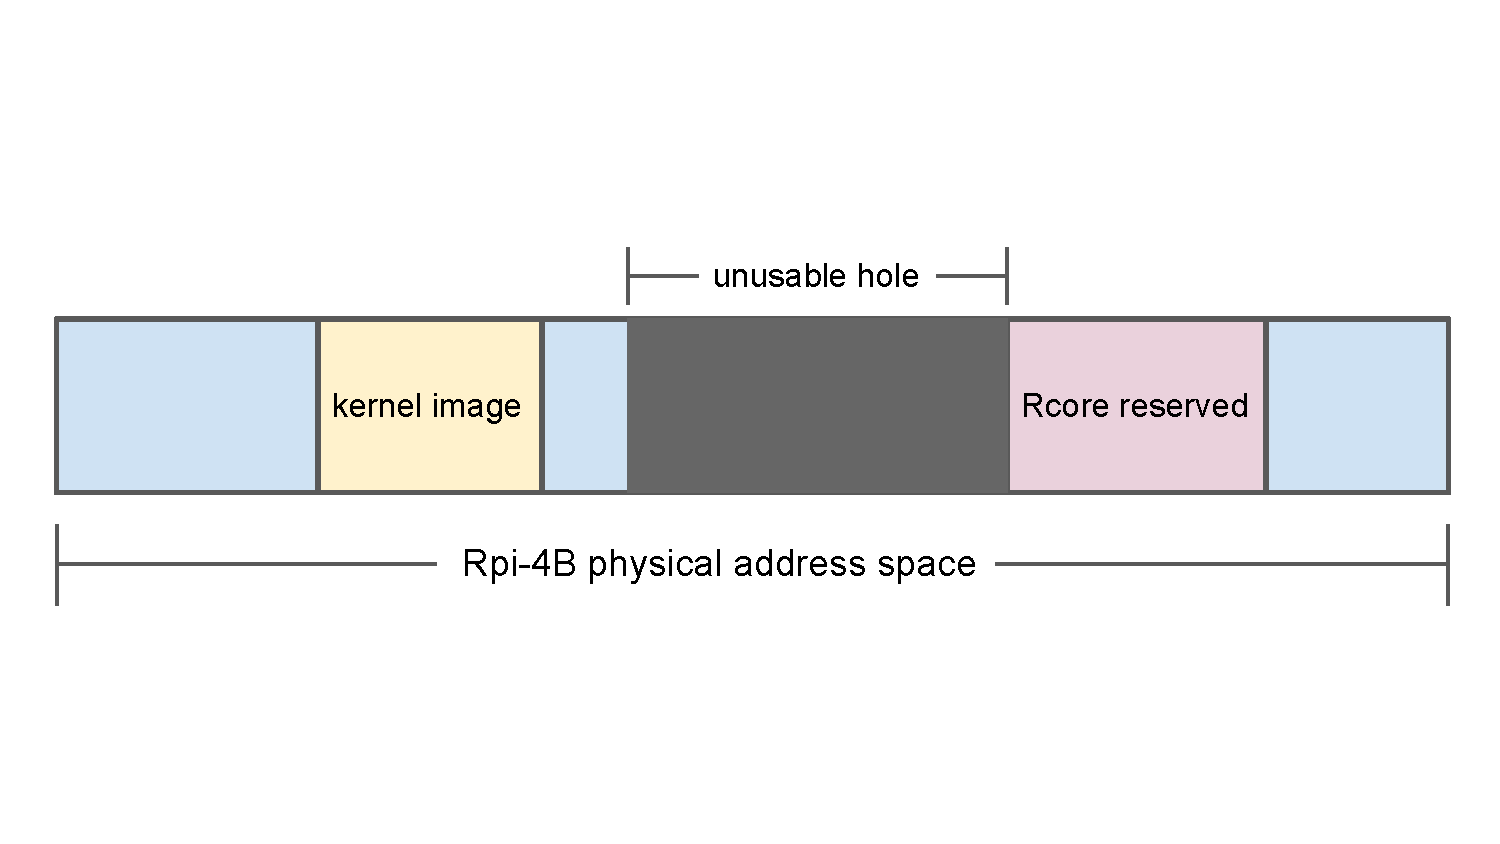
\includegraphics[scale=0.60]{figures/rcore_reserved.pdf}
    \caption{Overlap prevention}
    \label{fig:rcorereserved}
\end{figure}

\section{Rewriting C-based \secore{} into Rust-based \rustcore{}}

%challenge: difficult to do a top-down design due to the difficulty to debug
%and complexity of a hypervisor (is this challenge kinda weak?)
%
%solution: two pass method, first function-by-function rewrite, then remove
%unsafe and redesign after we have a working Rust hypervisor, and leverage
%Rust to achieve a stronger memory region isolation guarantee.

Given the high complexity of the KVM hypervisor and \secore{},
it is clear from the beginning that
a top-down approach to a Rust rewrite would be error-prone and difficult to test.
Therefore, we elected to start the rewriting effort bottom-up,
where all previous C functions are rewritten in Rust, one by one.
This incremental approach allows us to test our progress of function rewrite in
succession, reducing the risk of introducing bugs.
%One major downside of this approach is that it is difficult to rewrite a single
%function in a Rust-idiomatic and safe way.
One major downside of this approach is the difficulty of rewriting individual
functions in a manner that adheres to Rust's idiomatic practices.
Furthermore, it may result in a lot of \code{unsafe} blocks.
We solve these issues by adding a second phase to the Rust rewrite;
after the initial function by function rewrite, we removed unnecessary
\code{unsafe} blocks, refactored the code to be more Rust-idiomatic,
and leveraged Rust's type system to let Rust automatically check for safety
properties.

We discuss the usage of the type system to secure \rustcore{} in
\autoref{sec:securercore}.
